\newif\ifENG
\ENGtrue % 英語版を使用する場合はtrue、和文版を使用する場合はfalseに設定

\documentclass{article}
\usepackage[paperwidth=84.1cm, paperheight=118.9cm, margin=0cm]{geometry}
\usepackage{tikz}
\usepackage{graphicx}
\usepackage{fontspec}

% 色の定義
\definecolor{mydeepblue}{HTML}{332E83}

% 背景用
\definecolor{deepBackground}{HTML}{332E83} % 深い藍(背景など)
\definecolor{softGray}{HTML}{CCCCCC}       % 淡い灰色(背景補助)
\definecolor{lightIvory}{HTML}{F8F5E1}     % 生成的な淡ベージュ

% タイトル・見出し用
\definecolor{katanoPurple}{HTML}{4B0082}   % 目立つ紫
\definecolor{katanoBlue}{HTML}{4466CC}     % 明るい青
\definecolor{katanoIndigo}{HTML}{3A4F92}   % 落ち着いた藍
\definecolor{katanoBrown}{HTML}{5C4033}    % 和風の焦げ茶

\definecolor{katanoMediumOrchid}{HTML}{BA55D3} % 明るい紫、ピンクがかる
\definecolor{katanoMediumPurple}{HTML}{9370DB} % 少し青みが強い
\definecolor{katanoOrchid}{HTML}{DA70D6}       % さらに明るいピンク寄り
\definecolor{katanoViolet}{HTML}{EE82EE}       % 淡い紫、明度が高い
\definecolor{katanoSlateBlue}{HTML}{6A5ACD} % くっきりめ紫
\definecolor{katanoPurpleStrong}{HTML}{6A5ACD} % SlateBlue系


\definecolor{katanoSlateBlue}{HTML}{6A5ACD} % 青紫・視認性良好
\definecolor{katanoMediumSlateBlue}{HTML}{7B68EE} % やや明るい青紫
\definecolor{katanoBlueViolet}{HTML}{8A2BE2} % かなり青い鮮やか紫

% 本文用
\definecolor{katanoTextGray}{HTML}{333333} % 濃い灰(本文)

\setmainfont{Noto Sans}
\newfontfamily\jpfont{Noto Sans CJK JP}

%\setmainfont{Noto Sans CJK JP} % 日本語フォントを指定

\pagestyle{empty}

\begin{document}

\begin{tikzpicture}[remember picture, overlay]

% 背景色
%\fill[blue] (current page.south west) rectangle (current page.north east);

% 背景画像(使う場合コメントアウトを外す)
%\node[anchor=south west, inner sep=0] at (current page.south west) {
%  \includegraphics[width=\paperwidth,height=\paperheight]{background.jpg}
%};

% 背景画像をページ全面に敷く
\node[
  anchor=south west,
  inner sep=0,
  opacity=0.2, % 透明度を設定
] at (current page.south west) {
  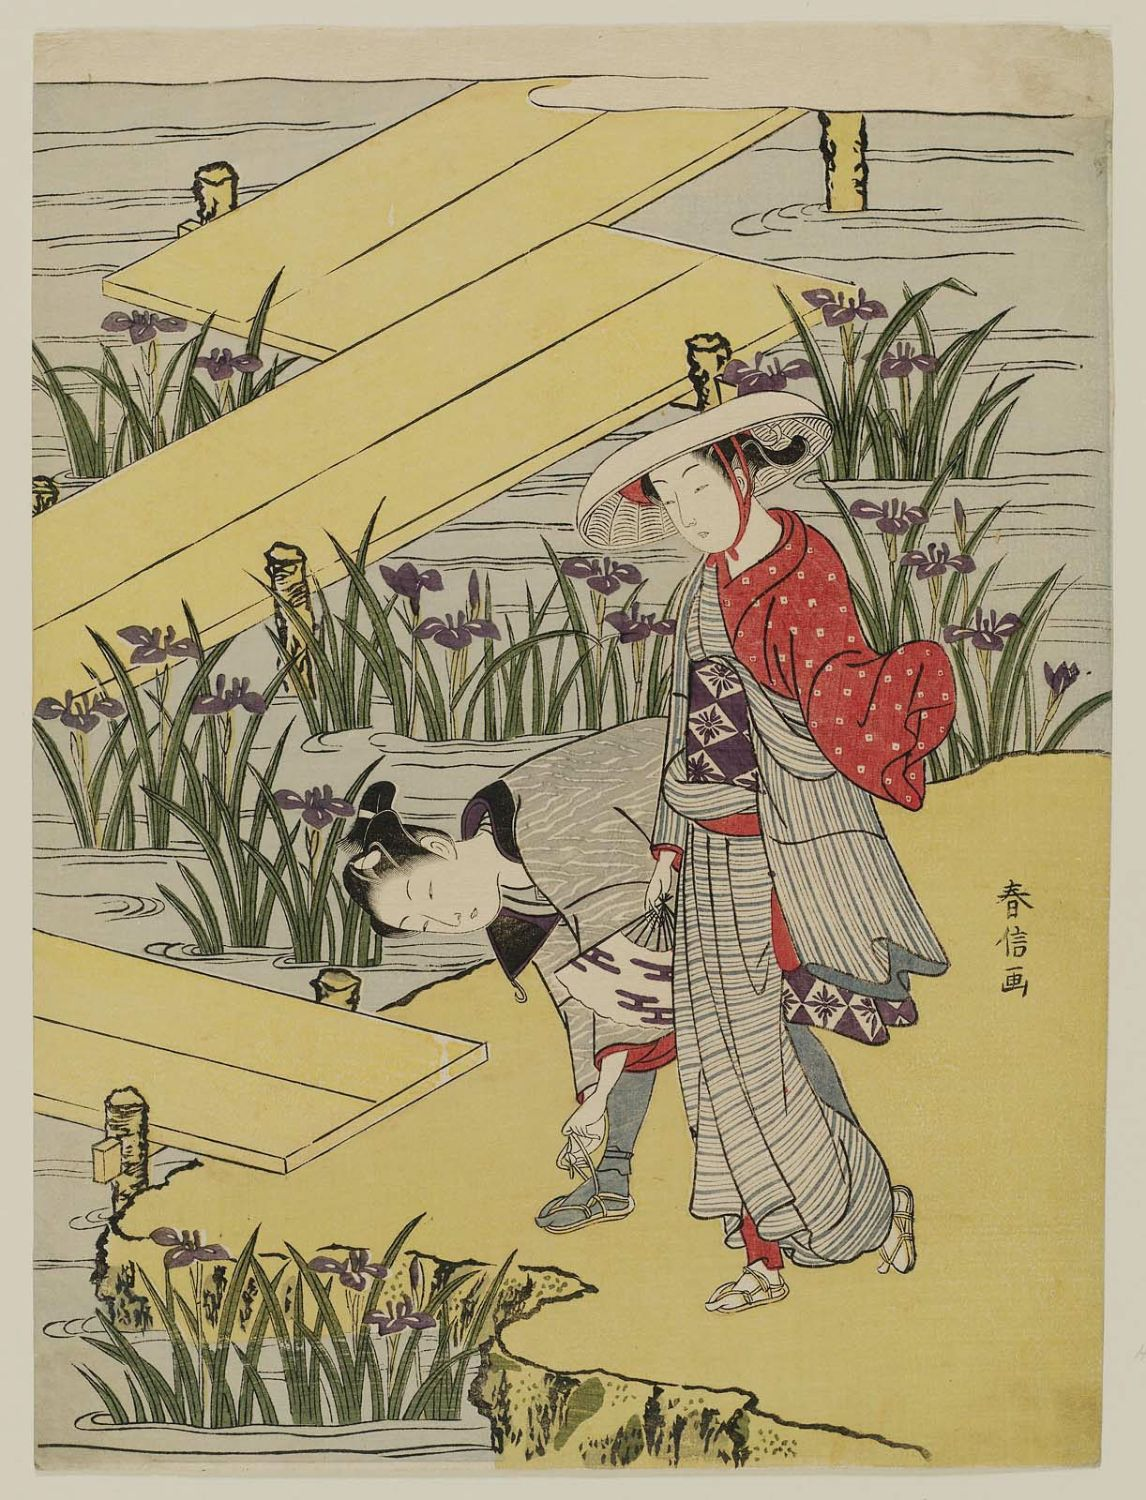
\includegraphics[width=\paperwidth,height=\paperheight]{
%  ise-katano.jpg
    images/yatsuhashi.jpg
}
};

% 画像の著作権
\node[
  anchor=north west,
  align=left,
  color=katanoMediumPurple,
  font=\fontsize{20pt}{20pt}\bfseries
] at ([xshift=1cm,yshift=2cm]current page.south west) {
\ifENG
% Background: Katano; Admiring the Scattered Cherry Blossoms
Background Image courtesy of the Museum of Fine Arts, Boston; Public Domain
%  \jpfont{画像提供:\textbf{いせかたの}(伊勢物語のカタノ)}
\else
画像出典:ボストン美術館(パブリックドメイン)
\fi
};

% Title
\node[
  anchor=north,
  align=center,
  text=blue!80!black,
  font=\fontsize{60pt}{70pt}\bfseries
] at ([yshift=-2cm]current page.north) {
  Translating Ise Monogatari through the Lens of Process Grammar Model
};

% Subtitle
\node[
  anchor=north,
  align=center,
  text=mydeepblue,
  font=\fontsize{60pt}{70pt}\bfseries
] at ([yshift=-5cm]current page.north) {
  A Bilingual and Structured Approach to Classical Japanese Narratives
};

% Authors
\node[
  anchor=north,
  align=center,
  font=\fontsize{50pt}{40pt}\bfseries
] at ([yshift=-8cm]current page.north) {
Hilofumi Yamamoto{\raisebox{1.5ex}{\fontsize{20pt}{20pt}\selectfont 1}}
\quad
Bor Hodošček{\raisebox{1.5ex}{\fontsize{20pt}{20pt}\selectfont 2}}
\quad
Xudong Chen{\raisebox{1.5ex}{\fontsize{20pt}{20pt}\selectfont 1}}
};

% 所属
\node[
  anchor=north,
  align=center,
  font=\fontsize{40pt}{30pt}\bfseries
] at ([yshift=-11cm]current page.north) {
{\raisebox{1.5ex}{\fontsize{20pt}{20pt}\selectfont 1}}
Institute of Science Tokyo
\quad
{\raisebox{1.5ex}{\fontsize{20pt}{20pt}\selectfont 2}}
The University of Osaka
};

% 左上テキストボックス
\node[
  draw=katanoBlue,
  line width=3pt,
  inner sep=10mm, 
  anchor=north west,
  text width=35cm,
  align=left,
  text=mydeepblue,
  font=\fontsize{30pt}{20pt}\bfseries
] at ([xshift=4cm,yshift=-15cm]current page.north west) {
  \textbf{\fontsize{40pt}{30pt}\selectfont Background}\\[1em]
  \textcolor{katanoBrown}{This section describes the background of the research...}
};

% 右上テキストボックス
\node[
  draw=katanoBlue,
  line width=3pt,
  inner sep=10mm, 
  anchor=north east,
  text width=35cm,
  align=left,
  text=mydeepblue,
  font=\fontsize{30pt}{20pt}\bfseries
] at ([xshift=-3cm,yshift=-15cm]current page.north east) {
  \textbf{\fontsize{40pt}{30pt}\selectfont Methods}\\[1em]
  \textcolor{katanoBrown}{Here you explain your methods in detail...}
};

% 中央下テキスト
\node[
  draw=katanoBlue,
  line width=3pt,
  inner sep=10mm, 
  anchor=north west,
  text width=75cm,
  align=left,
  text=mydeepblue,
  font=\fontsize{30pt}{20pt}\bfseries
] at ([xshift=4cm, yshift=-40cm]current page.north west) {
  \textbf{\fontsize{40pt}{30pt}\selectfont Results and Conclusion}\\[1em]
  \textcolor{katanoBrown}{Summarize the results and main findings here...}
};


% 中央下右テキスト
\node[
  draw=katanoBlue,
  line width=3pt,
  inner sep=10mm, 
  anchor=north west,
  text width=75cm,
  align=left,
  text=mydeepblue,
  font=\fontsize{30pt}{20pt}\bfseries
] at ([xshift=4cm, yshift=-80cm]current page.north west) {
  \textbf{\fontsize{40pt}{30pt}\selectfont Resources}\\[1em]
  \textcolor{katanoBrown}{Zenodo repository: \texttt{https://zenodo.org/record/1234567}}\\
};



% ロゴ(右下)
\node[
  anchor=south east
] at ([xshift=-1cm,yshift=1cm]current page.south east) {
  
\includegraphics[height=4cm]{images/sciencetokyo.png}
  
\includegraphics[trim=30 30 30 30, clip, height=4cm]{images/theUnivOsaka.jpg}
};

\end{tikzpicture}

\end{document}



